\subsection{Financial models of communication}

Late to a meeting is theft, and poorly written email and email to the wrong people has financial cost.

\subsubsection{Meeting time compared to theft}
% https://graphthinking.blogspot.com/2021/02/organizations-value-things-more-than.html

In large organizations, there can be significant bureaucracy associated with even small purchases. A multi-step review process may be incurred for a \$2000 acquisition.

Another measurement of value is that if an employee were to steal even \$200 worth of materials, the organization would likely punish that employee.


In the book High Output Management \cite{1995_Grove}, Grove points out that those metrics apply to tangible goods, but not to people's time. Consider a meeting of 10 people and each person's cost is \$200 per hour. A wasted meeting is not unusual and certainly would not incur bureaucratic review processes. The cost to the organization is fiscally the same -- \$2000. Similarly, consider an employee who is late and causes a loss of productivity. Merely depriving the organization of \$200 worth of time is not punished in the same way theft is.

In fact, organizations default to meetings (even recurring meetings) rather than not meet. And being late to a meeting is accepted. 

We can debate the differences between theft of materials and theft of time. The financial argument is clear. 


\subsubsection{Email is not free}

Total cost of email:
* time spent writing
* time spent reading
* infrastructure maintenance

Cost per email = 
(hourly rate of writer)*(time spent writing) + (hourly rate of reader)*(time spent reading)*(number of readers)+(annual salary of maintainer)/(number of emails per year) + (email server cost)/(number of emails per year), etc

50*(5/60) + 50*(5/60)*4 + 100000/1000000 + 10000/1000000 = \$21 for one email. 

\begin{figure}
    \centering
    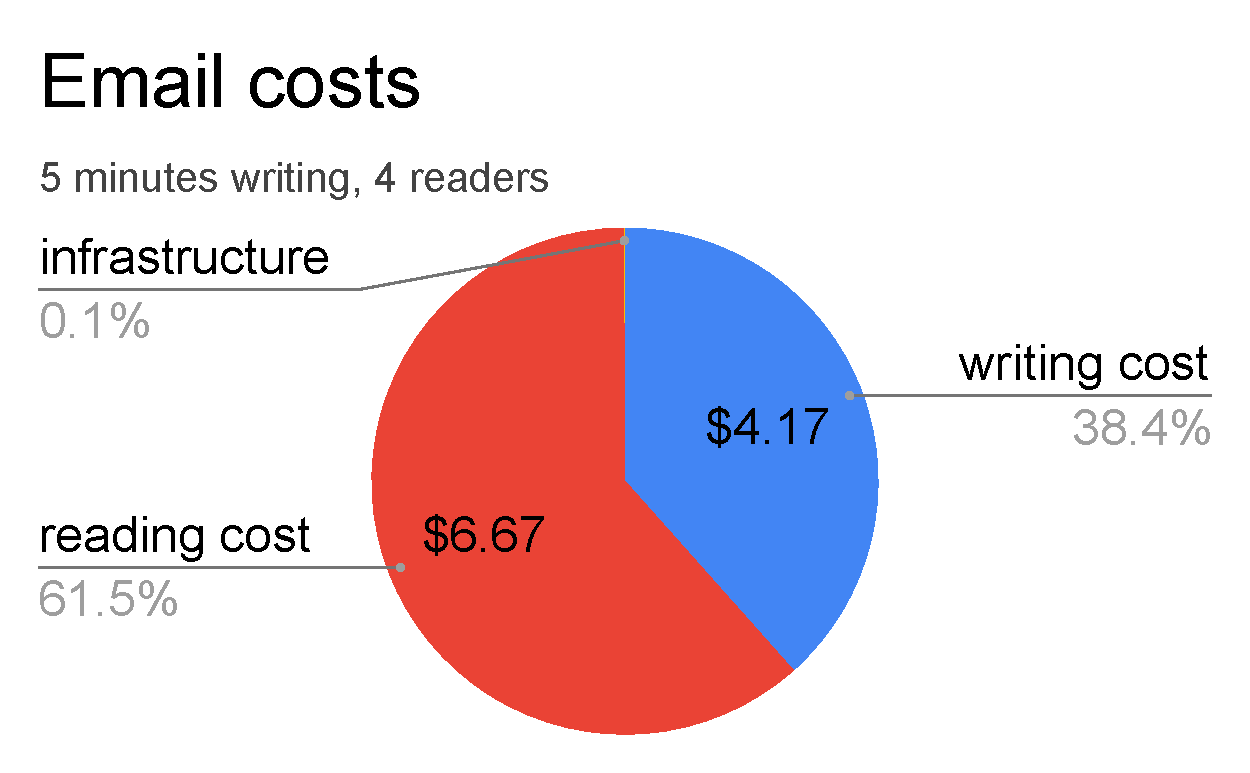
\includegraphics{images/email_costs_5minutes_4people.pdf}
    \caption{If email is 2 hours a day, and staffing is 50\% of the organizations budget, then 
    % (2/8)*0.5
    12.5\% of the organization's budget is spent on email. Same math for meetings, so that's 25\% of the organization's budget on coordination.}
    \label{fig:my_label}
\end{figure}

% https://docs.google.com/spreadsheets/d/1ysV5PA3cEcneKv5BViUhAfgNq26cOlNRj6l5fXuHM3Q/edit?usp=sharing

Paradigm for reading emails
* Unread
* Does this message have any bearing on my current task? 
* Integrate with my understanding 